\documentclass[a4paper,12pt]{article}

%===================================================================================
% Paquetes
%-----------------------------------------------------------------------------------
\usepackage{amsmath}
\usepackage{float}
\usepackage{amsfonts}
\usepackage{amssymb}
\usepackage[utf8]{inputenc}
\usepackage{listings}
\usepackage[pdftex]{hyperref}
\usepackage{graphicx}

\usepackage{listings}
\usepackage{color}

\definecolor{dkgreen}{rgb}{0,0.6,0}
\definecolor{gray}{rgb}{0.5,0.5,0.5}
\definecolor{mauve}{rgb}{0.58,0,0.82}

\lstset{frame=tb,
  language=Prolog,
  aboveskip=3mm,
  belowskip=3mm,
  showstringspaces=false,
  columns=flexible,
  basicstyle={\small\ttfamily},
  numbers=none,
  numberstyle=\tiny\color{gray},
  keywordstyle=\color{blue},
  commentstyle=\color{dkgreen},
  stringstyle=\color{mauve},
  breaklines=true,
  breakatwhitespace=true,
  tabsize=3
}

%-----------------------------------------------------------------------------------
% Configuración
%-----------------------------------------------------------------------------------
\hypersetup{colorlinks,%
	    citecolor=black,%
	    filecolor=black,%
	    linkcolor=black,%
	    urlcolor=blue}


\begin{document}

 

\title{ej6}

\begin{titlepage}
\centering
\vspace*{\fill}
\vspace*{0.5cm}
\huge\bfseries
HIVE\\
\vspace*{0.5cm}
\large Rodrigo García Gómez CC-412 \\ Jorge Mederos Alvarado CC-412
\vspace*{\fill}
\end{titlepage}


\section*{Instrucciones de uso}
Para ejecutar el juego debe importarse desde la terminal de swi-prolog el archivo main.pl.\\

\texttt{?- [main].} \\

Luego basta con usar el predicado run() para que aparezca en la pantalla el menú principal como se muestra en la figura 1.\\

\texttt{?- run().}\\

\begin{figure}[H]
	\centering
	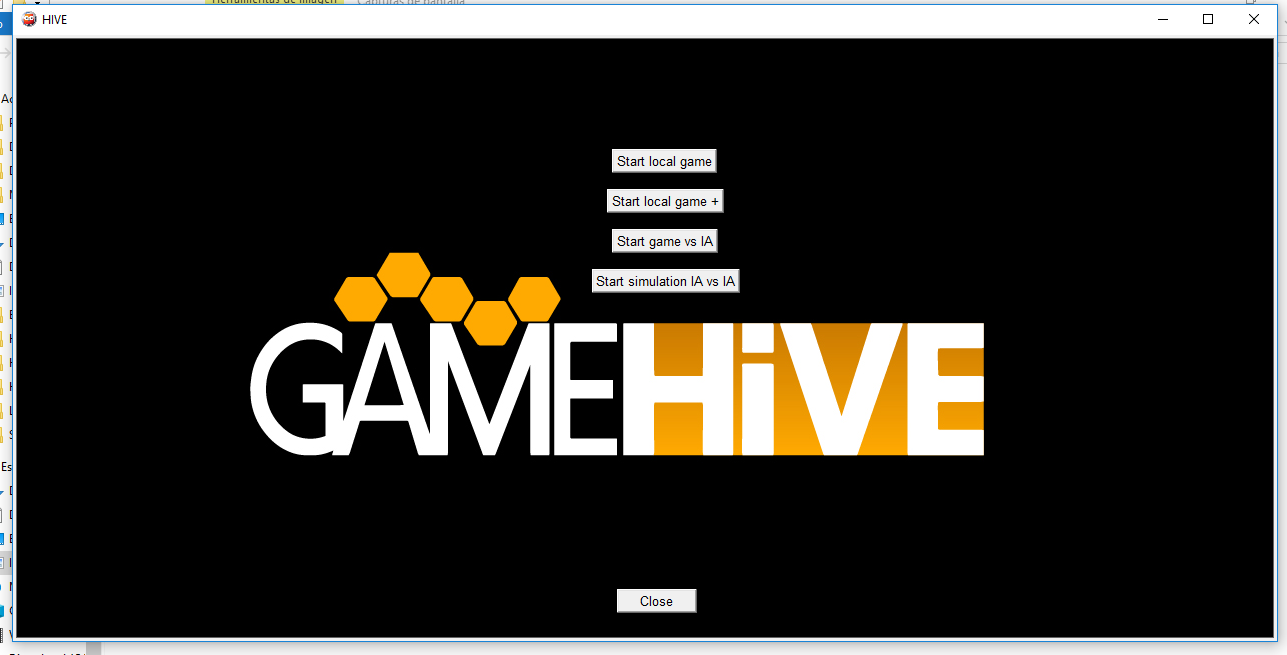
\includegraphics[width=0.9\linewidth]{./1}
	\caption{Menú Principal}
	\label{fig:1}
\end{figure}

Se muestran cuatro formas de juego distintas:

\begin{enumerate}
\item Start local game\\
Modo de juego local simple para dos jugadores. Cada jugador mueve las fichas haciendo click en las de su respectivo color. El jugador de las fichas negras siempre comienza. Se muestran sólo los 5 tipos de fichas del juego clásico: reina, hormiga soldado, saltamontes, escarabajo y araña.

\item Start local game +\\
Modo de juego local expandido. Al igual que el primer modo, este es para dos jugadores. Se agregan tres tipos de fichas: la mariquita, el mosquito y el bicho bola.

\item Start game vs IA\\
Este modo es para un jugador. El usuario controlará las fichas negras. Luego de hacer cada jugada, la pc responderá con otra. Se muestran primero las opciones de movimiento de la ficha seleccionada por la IA y acto seguido, esta es desplazada a la posición escogida.

\item Start simulation IA vs IA\\
Modo de juego expectador. El usuario podrá presionar el botón "Play" para que la pc realice la siguiente jugada escogida. Doble click en el botón mostrará las opciones de movimiento de la ficha escogida en cada momento antes de esta ser desplazada.
\end{enumerate}

La figura 2 muestra una vista general del tablero.

\begin{figure}[H]
	\centering
	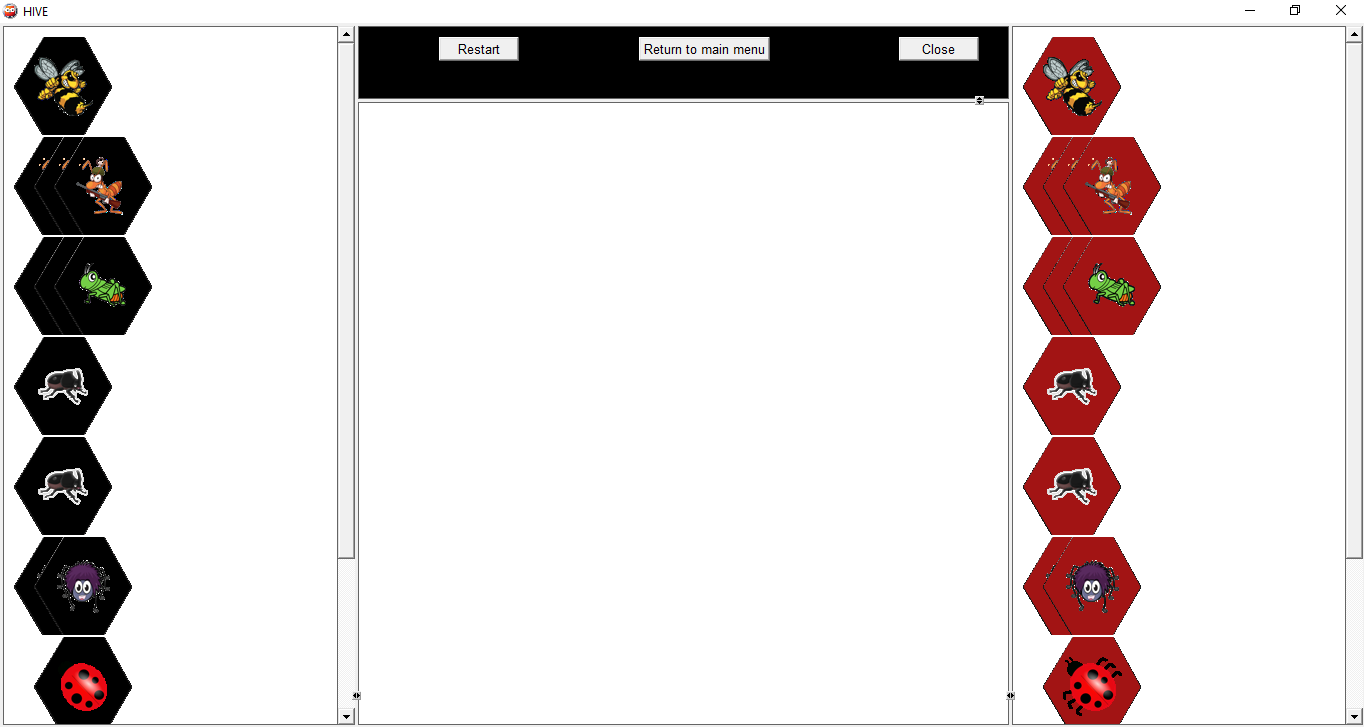
\includegraphics[width=0.9\linewidth]{./2}
	\caption{Tablero de juego}
	\label{fig:2}
\end{figure}

Las fichas del jugador negro y rojo se muestran en ventanas a la izquierda y derecha respectivamente. Al hacer click sobre una ficha durante tu turno, se mostrarán hexágonos grises en todas las posiciones accesibles por dicha ficha. Tocar uno de estos hexágonos hará que la ficha seleccionada se desplace a la posición del hexágono. Los escarabajos (y los mosquitos a veces) tienen la habilidad de caminar por encima de las fichas y evitar que estas puedan realizar acciones; cuando un escarabajo se posiciona sobre una ficha, esta pasa a mostrarse en la posición inicial de dicho insecto. Cuando el escarabajo se mueve, las fichas posicionadas debajo suyo vuelven a mostrarse en su respectiva posición.\\
En la parte superior del tablero se encuentra un menú con tres opciones. "Restart" reiniciará el juego en el modo actual. "Return to main menu" cerrará la ventana de juego y abrirá nuevamente el menú principal. "Close" dará por cerrada la aplicación.

\section*{Detalles de implementación}
\subsection*{Interfaz gráfica}
Se utilizó la librería xpce para manejar todo lo relacionado con la graficación del juego. En el script main.pl se maneja el código relacionado con esta librería. Todas las imágenes son importadas como recursos mediante: 

\texttt{\\:- pce\_image\_directory('./').\\ resource(name, image, image('archive')).} \\

A partir de este punto, la palabra name estará asociada a la imagen de nombre 'archive' ubicada en la dirección donde se encuentra el script main.\\
XPCE permite la creación de variables de la forma @nombre que son accesibles desde cualquier sección del código. Sin embargo, esas variables tienen el inconveniente de que en caso de no liberarse entre una ejecución y otra, provocarán un error al volver a crearlas. Al ejecutar run/0, se ejecuta a su vez free\_all/0 para liberar cualquier variable que pueda haber quedado en ejecuciones anteriores, en caso de que el juego se haya cerrado mediante un método diferente del botón "Close". Luego se ejecutará main/0 para crear el objeto "Frame" que tendrá la ventana del menú principal y los objetos "Button" de los distintos modos de juego. Al escoger un modo de juego se cierra el menú y se abre un nuevo "Frame" acorde al modo escogido (La única diferencia visual entre los modos de juego es el botón "Play" para el modo simulación).\\
El tablero de juego está conformado por un objeto "Picture" (@board) en el centro, dos objetos "Window" a su izquierda (@left\_window) y derecha (@right\_window) para las posiciones iniciales de las fichas y una ventana superior (@menu) para el menú de opciones. Al guardar cada objeto en una variable @ de XPCE, se facilita el acceso a ellos para desplazar las piezas del juego. Las fichas son objetos "Device" con imágenes de tipo "Bitmap" agregadas. Al hacer click sobre la imagen de un insecto, se envía un mensaje a @prolog para ejecutar el predicado que buscará las posiciones disponibles para cada caso y creará en estas otro "Device" con la imagen de un hexágono gris. Estos hexágonos grises tendrán a su vez sus recognizer de "click\_gesture" para detectar click sobre ellos y desplazar hacia su posición a la última ficha seleccionada. Todos los hexágonos grises son limpiados al mover una ficha.\\
Cuando se detecta mediante check\_for\_lose() que una de las dos reinas se encuentra rodeada, se abre una ventana con la imagen "Game Over" para anunciar el final del juego. A partir de este punto el funcionamiento de las fichas se desactiva y se espera a que el usuario presione alguno de los botones del menú superior.\\
Los botones "Close" del menú superior y del menú principal liberarán todas las variables @.\\
Los predicados más importantes de XPCE son "new", que se utiliza para crear objetos nuevos; "send" que envía información a los objetos y "get" utilizado para objeter información de estos. Al enviar display a una "Ventana" o "picture", se envía la orden de mostrar esa ventana el objeto escogido. Además se puede enviar su ubicación cartesiana con un parámetro point(x,y). Esta ubicación además puede ser obtenida luego mediante un "get".\\

A continuación se muestra un ejemplo del uso de XPCE.\\

\begin{lstlisting}
initialize_bug(Window, Image, Hexagon, Pos, BugType, HexColor, OutBug):-
	new(OutBug, device),
	send(OutBug, name, BugType),
	new(Hex, bitmap(resource(Hexagon), @on)),
	send(OutBug, display, Hex, point(-20,-20)),
	new(Bug, bitmap(resource(Image), @on)),
	send(OutBug, display, Bug),
	send(Bug, recogniser, click_gesture(left, '', single, message(@prolog, select_bug, OutBug, HexColor))),
	send(Window, display, OutBug, Pos).
\end{lstlisting}

Se crea un "Device" de nombre OutBug, se le agregan los bitmap de hexágono y e imágen de insecto, se le agrega el recognizer que llama a select\_bug cuando se presiona la imagen del insecto y se le envía display a la ventana seleccionada.

\subsection*{Implementación de reglas y lógica general}
Las fichas de los insectos están vinculadas a select\_bug(Bug, HexColor). Este predicado analiza la situación del tablero y las características del insecto "Bug" para generar en el tablero los hexágonos grises correspondientes. La variable bugs (variable global accedida mediante nb\_getval/2) es una lista de listas de la forma [Bug, Color] que mantiene un rastreo de todas los insectos que ya han sido colocados en el tablero. Ademásn turn\_count mantiene un contador que aumenta en uno con cada jugada hecha y turn tiene "red" o "black" en dependencia de cuál fue el último lado que movió ficha. Primeramente se revisa si el color del turno actual no coincide con el color de la ficha a la que se hizo click, en cuyo caso el predicado triunfa sin llegar a generar ningún hexágono gris. Lo mismo pasa si la ficha tocada está actualmente debajo de un escarabajo (esto se revisa con check\_all\_stacks/2 que recibe como primer parámetro el insecto a revisar y devuelve en el segundo qué escarabajo o mosquito lo tiene tapado en caso de triunfo. Si no está tapado por ningún escaabajo o mosquito, falla) o si fue movida en el turno anterior por un bicho bola (esto último se almacena en la variable "last"). Además, en caso de estar en el tercer turno del jugador negro o rojo y de que aún su respectiva reina no haya sido colocada en el tablero, también se triunfa sin generación de hexágonos siempre que la ficha seleccionada no sea la reina que debe colocarse. Luego se pasa a objtener la lista de listas con forma [[x,y]|Tale] que tiene todas las posiciones a las que se puede mover el bicho seleccionado. Esto puede hacerse de tres formas: En caso de ser la primera jugada, sólo estará la posición central del tablero; en caso de no ser la primera jugada, pero de ser un insecto que aún no ha sido colocado en el tablero, se ejecuta el predicado new\_bug/1, que retorna en su parámetro la lista con las posiciones que bordean a las fichas del color del turno actual y que no colindan con ninguna del color contraio; En caso de que el insecto clickeado sea uno ya colocado en el tablero, se invocará el predicado correspondiente a su tipo (el funcionamiento de estos se explicará a detalle más adelante). fill\_with\_gray/3 creará un device hexágono gris en cada una de las posiciones que pertenezcan a la lista pasada como parámetro.\\
Los hexágonos grises tendrán como recognizer de click\_gesture otro predicado importante: move\_bug\_to\_position/4 que recibe el insecto a mover, la posición a donde se quiere desplazar (que es la posición del hexágono que lo invoca) y el color de este insecto. Este predicado se importa desde el script bug\_movement y triunfa luego de desplazar la ficha en cuestión. En caso de la ficha no estar agregada anteriormente al tablero, también la incluye en la lista "bugs". Además actualiza el contador de turnos y la variable "turn" con el úlimo color jugado, limpia los hexágonos grises del tablero y revisa a ambas reinas en busca de una condición de fin de juego. Stack\_bug/3 revisa si la posición a donde se quiere mover la ficha está ya ocupada, en cuyo caso esta debe ser un escarabajo o un mosquito y se guarda en su respectiva pila a la pieza ocupando esta posición para saber que se encuentra debajo del escarabajo o mosquito. Hay 6 pilas en total: bb1, bb2, rb1, rb2, bm y rm; una para cada insecto con la abilidad de pasar por encima de otros. La invocación de move\_IA/1 se explicará más adelante.


\section*{Obtención de movimientos de fichas}
Cada tipo de insecto tiene su propio movimiento vinculado. La implementación de estos movimientos está en los script con los nombres de sus respectivas especies. En todos los casos se ejecuta check\_conex/3 que realiza un DFS simple para revisar las posiciones obtenidas y eliminarlas en caso de que desconecten la colmena.

\begin{enumerate}
\item queen/2\\
Recibe a la reina en cuestión y retorna las posiciones disponibles. Calcula las 6 posiciones colindantes con la de la reina y para cada una invoca el predicado try\_add\_free\_position/6. Este recibe la actual lista de posiciones libres como segundo parámetro y retorna en el 4to parámetro la lista actualizada que puede tener o no agregada la posición pasada como primer parámetro en caso de esta no estar previamente en la lista o de pertenecer a la lista de posiciones ocupadas del tercer parámetro. El 5to y 6to parámetro tiene las dos posiciones que quedan a la izquierda y derecha de la posición a revisar (viéndola desde la posición de la reina); en caso de estar ocupadas las dos, la reina tampoco podrá pasar, pues no la ficha no tendrá espacio para deslizarse (esta regla no sale en la orientación del proyecto, pero fue incluida en la implementación por estar presente en varias versiones de las reglas de HIVE).

\item grasshopper/2\\
Recibe saltamontes y retorna posiciones disponibles. Es parecido al predicado de la reina, con la diferencia de que en lugar de try\_add\_free\_position/6, invoca a try\_jump\_in\_direction/7. Se revisa recursivamente en línea recta por las posiciones ocupadas del tablero a partir de la primera ocupada en la dirección específicada. Al encontrar una posición no ocupada, es agregada a la lista que se recibe en el segundo parámetro y se retorna en el cuarto, siempre que esta posición desocupada no esté colindante con el saltamontes sin ninguna otra ficha por el medio. En caso de no agregar ficha, se triunfa igualmente retornando la lista sin modificar.

\item ant/5\\
se recibe como primer parámetro una lista que inicialmente sólo tendrá [x,y], la posición de la hormiga. el segundo y tercer parámetro son también la X y la Y, posiciones de la hormiga para poder luego retirarla del grafo de posiciones ocupadas y realizar el check\_conex. El 4to y 5to parámetro son la lista recibida por la iteración anterior (inicialmente vacía) y su actualización con la iteración actual. Se actualiza recursivamente el primer parámetro con todas las posiciones agregadas a la lista de posiciones disponibles (que se revisan con try\_add\_free\_position/6) durante la iteración actual para luego reviar a partir de estas sus posiciones disponibles adyacentes. Cuando la lista del primer parámetro está vacía al no quedar posiciones para agregar, entonces se llega al caso base y se retorna la solución en el 5to parámetro.

\item spider/8\\
El funcionaminto de este predicado es parecido al de la hormiga. La diferencia es que lleva un contador en el 4to parámetro que decrece en uno acorde a la profundiad del llamado recursivo. Además, tiene los parámetros 7 y 8 en los que se recibe y se retorna la lista de la solución. al llegar a profundidad 3, se actualiza esta lista y se llega al caso base. Al terminar todos los llamados recursivos, el 8vo parámetro tendrá todas las posiciones de profundidad 3 a partir de la posición de la araña, tal que no estén ocupadas y no desconecten la colmena.

\item bitle/2\\
Esta ficha se mueve parecido a la reina. Al igual que esta, recibe como primer parámetro al insecto en cuestión y retorna en el segundo la lista de posiciones disponibles para movers. La diferencia está en que la lista pasada como tercer parámetro de try\_add\_free\_position/6 siempre estará vacía, pues el escarabajo se puede mover también a las posiciones ocupadas, y los parámetros 5 y 6 tendrán posiciones inaccesibles ya que estas no importarán. Para revisar la posible desconexión del grafo se revisa el stack del escarabajo, puesto que si se encuentra sobre otro insecto, al moverse nunca desconectará la colmena.

\item ladubyg/8\\
La implementación de este predicado es muy similar a la de la araña. La diferencia está en que durante la profundiad 1 y 2 se camina sólo por las posiciones ocupadas con ladybug\_try\_add\_free\_position/4 y cuando se alcanza la profundidad 3, se agragan las posiciones que no están ocupadas y estas son las que se agregan a la lista de retorno.

\item mosquito/2\\
El mosquito, en lugar de agregar posiciones a su alrededor, invoca al predicado mosquito\_copy\_in\_direction/5 para cada una de sus posiciones adyacentes. Para cada posicion que esté ocupada por otra ficha, invoca su respectivo predicado y obtiene las posiciones imitando su comportamiento. En el segundo parámetro se retorna la unión de las posiciones devueltas por cada imitación de comportamiento. El tener algo en su pila, implica que el mosquito se encuentra actualmente sobre otra ficha, en cuyo caso sólo podrá moverse como un escarabajo.

\item pillbug/3\\
El poderoso bicho bola, al igual que la reina y el escarabajo, revisa sus posiciones adyacentes. Pero en lugar de try\_add\_free\_position/6, invoca pillbull\_try\_add\_free\_position/8, una versión propia. En caso de estar desocupada la posición, entonces se actúa como el predicado normal. La diferencia está en las posiciones ocupadas	Primeramente se revisa que la ficha que esté ocupando la posición no sea la almacenada en la variable ´"last" o que no sea un insecto apilado, en cuyo caso se retorna la lista de posiciones sin modificar. En caso contrario, sobre la posición ocupada se colocará un hexágono especial que en ligar de tener asociado al recognizer el predicado move\_bug\_to\_position/4, tendrá pillbug\_select\_bug\_to\_move/3. Este hexágono, al ser clickeado no moverá ningún insecto, sino que colocará nuevos hexágonos grises en las posiciones libres alrededor del bicho bola que asociarán su movimiento con el insecto de la posición clickeada.
\end{enumerate}

Todos estos predicados triunfan siempre, en caso de no haber posiciones disponibles para mover la ficha seleccionada, se retorna una lista vacía y por tanto no se crean nuvos hexágonos.

\subsection*{IA}
Al escoger el modo player vs IA, se le da valor 1 a la variable vs\_IA que es revisada por move\_bug\_to\_position/4 luego de que el jugador hace una jugada. Entonces se invoca a move\_IA/1 para que la PC juegue por las fichas rojas. En este punto se analizarán las posibles jugadas de cada ficha roja y se escogerá la mejor acorde a una puntuación otorgada. Esta puntuación estará influenciada por los pesos dados a cada criterio tomado en cuenta. Para cada ficha se escoge una jugada con mayor puntuación, luego se comparan las puntuaciones de la mejor jugada de cada ficha y la mayor entre todas es escogida para realizarse. Los criterios de puntuación para posibles jugadas varían entre insectos. A continuación se mencionan ejemplos de la heurística utilizada por el sistema de puntuación de cada jugada por los distintos insectos:\\
La ganancia de puntuación de las jugadas de la reina será inversamente proporcional a la cantidad de fichas que tenga alrededor la posición candidata y directamente proporcional a la cantidad de fichas que tenga alrededor la posición actual de la reina. De esta manera la reina siempre tratará de estar lo menos rodeada posble.\\
Una jugada de una hormiga ganará mayor puntuación si se encuentra adyacente a la reina rival y aún más si las otras dos posiciones que se encuentran adyacentes tanto a la hormiga como a la reina están vacías. De esta froma, la reina rival no podrá moverse sin desconectar la colmena.\\
Las jugadas del escarabajo serán mejor puntuadas de acuerdo a su distancia con respecto a la reina rival, mientras más cerca se mueva de esta, mejor. Además ganará puntos por posicionarse encima de fichas rivales y perderá puntos por posicionarse sobre fichas aliadas. También influye el rango de estas, posicionarse sobre una hormiga rival es mejor que sobre una araña rival; mientras que posicionarse sobre una hormiga aliada es peor que sobre una araña aliada.\\
También, tanto las jugadas candidatas de el escarabajo como del saltamontes ganarán mayor puntuación si se encuentran adyacentes a la reina rival, y mayor puntuación aún si están rodeadas por 5 o 6 fichas. Las posiciones rodeadas por 5 o 6 fichas no son accesibles por otras fichas y por tanto es importante rellenar esos agujeros adyacentes a la reina rival con las fichas que sí pueden acceder a ellos.\\
El movimiento de la araña es limitado, por lo que ganará una puntuación relativamente alta si logra colocarse adyacente a la reina rival. Además, las jugadas candidatas de la araña y de otras piezas como el saltamontes y el escarabajo ganarán puntos recursivos a una profundiad de hasta tres jugadas, con una penalización proporcional a la profundiad. Una jugada candidata de la araña ganará puntos si luego de realizarse, la araña puede moverse a una posición adyacente a la reina desde ella. Pero la puntuación que recibe por esto es la mitad de la que recibe una jugada por estar directamente adyacente a la reina rival. El análisis de jugadas a profundiad le brinda a la IA la oportuniad de posicionar sus piezas en posibles futuras buenas jugadas. No es necesario analizar profundiades mayores que tres pues es poco probable que la colmena se separe tanto que las fichas queden tan lejanas. Y en caso de que esto pasara, es mejor mover una que esté cerca antes de mover una que necesita de cuatro jugadas para hacer algo bueno.\\
Todas las puntuaciones de las jugadas candidatas reciben una penalización acorde a qué tan buena es su posición actual. Si un escarabajo se encuentra actualmente adyacente a la reina rival y apilado sobre una hormiga rival, aunque tenga otra hormiga rival adyacente para posicionarse sobre, no deberá moverse pues su posición actual es buena.\\
El tiempo de ejecución de la decisión de la IA es despreciable, pues la cantidad de fichas es constante y pequeña, al igual que la cantidad de jugadas posibles de estas. Analizar todas las posibles jugadas es instantáneo. Luego de decidida la jugada a realizar, el programa duerme durante un segundo, tiempo durante el cual se muestran los hexágonos grises que representan las posibles jugadas que la ficha escogida podía realizar. Luego, la ficha se desplaza a la posición escogida y nuevamente comienza el turno del jugador.
Al escoger el modo simulación, el usuario no participa. La PC juega por cada lado alternativamente cada vez que se presiona el botón "PLAY!".







\end{document}